% Created by tikzDevice version 0.9 on 2015-12-15 11:28:56
% !TEX encoding = UTF-8 Unicode
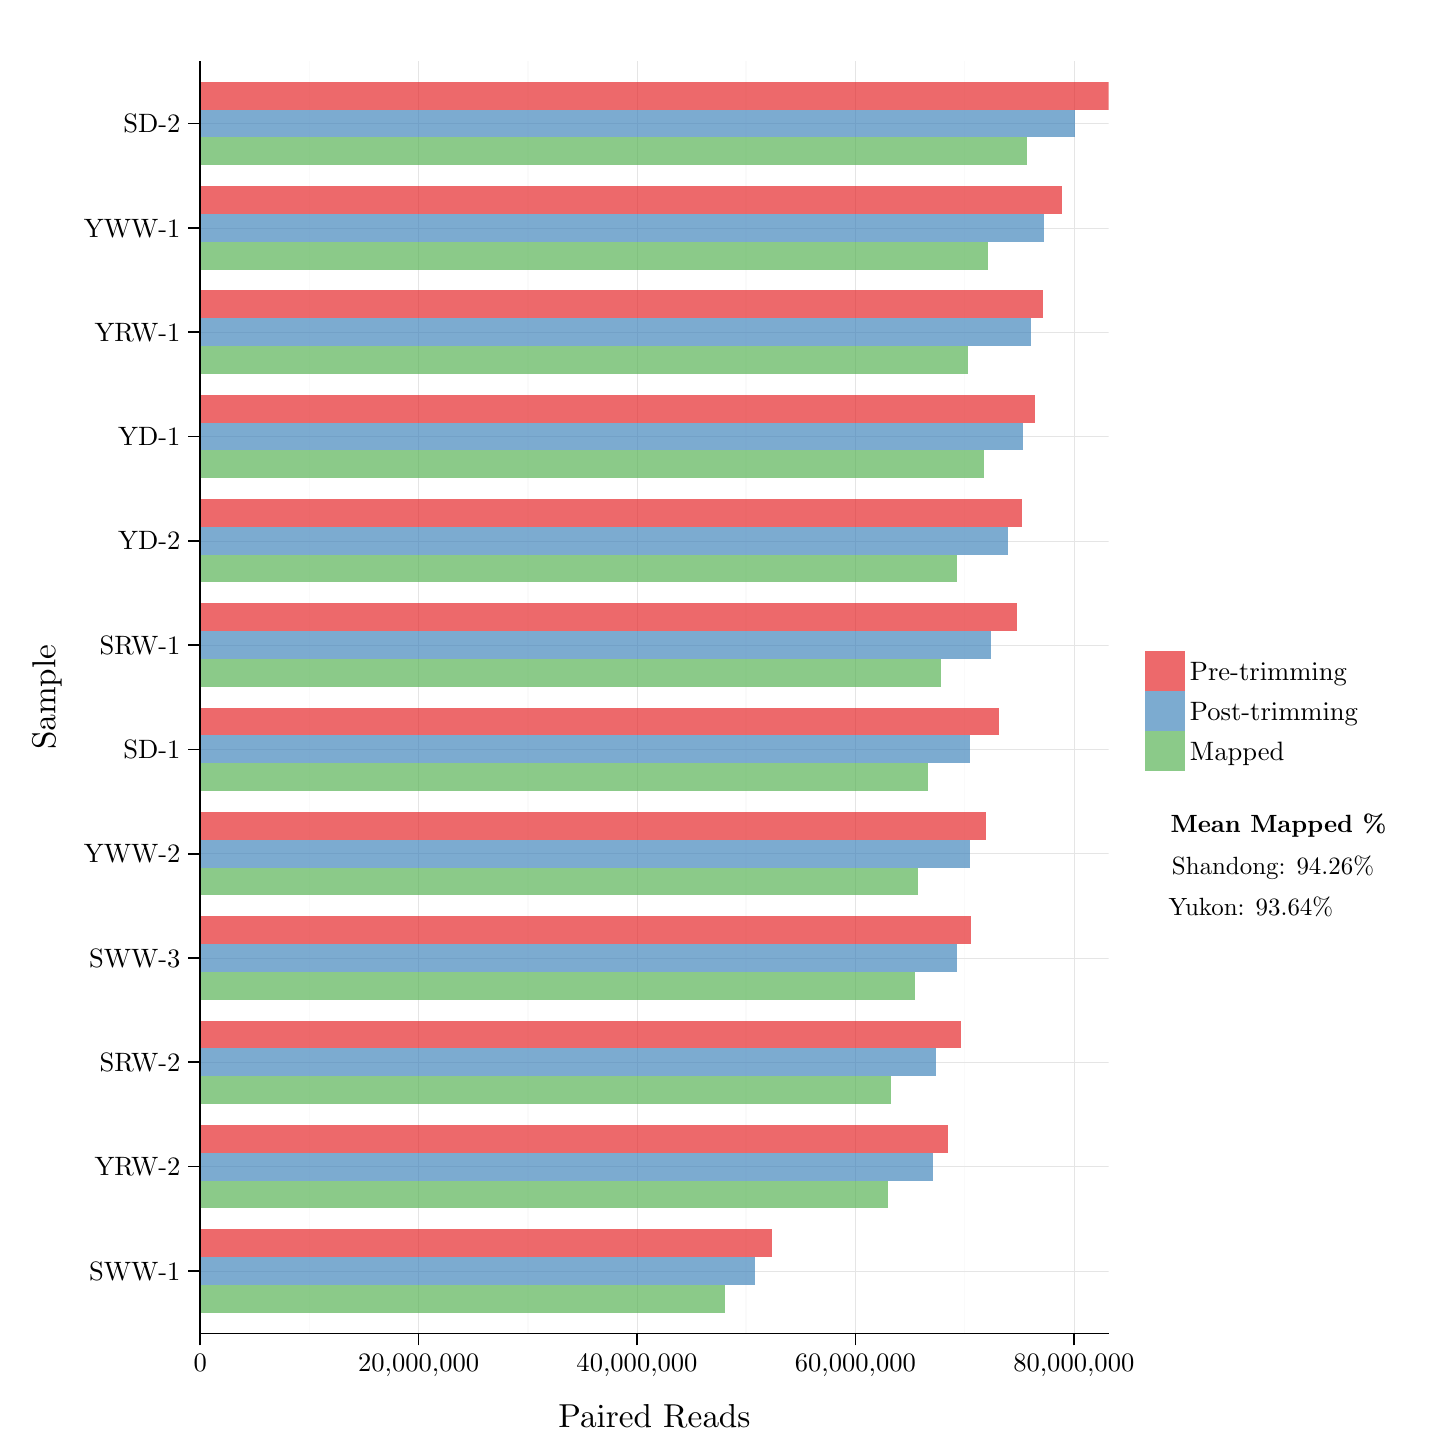
\begin{tikzpicture}[x=1pt,y=1pt]
\definecolor{fillColor}{RGB}{255,255,255}
\path[use as bounding box,fill=fillColor,fill opacity=0.00] (0,0) rectangle (505.89,505.89);
\begin{scope}
\path[clip] (  0.00,  0.00) rectangle (505.89,505.89);
\definecolor{drawColor}{RGB}{255,255,255}
\definecolor{fillColor}{RGB}{255,255,255}

\path[draw=drawColor,line width= 0.6pt,line join=round,line cap=round,fill=fillColor] (  0.00,  0.00) rectangle (505.89,505.89);
\end{scope}
\begin{scope}
\path[clip] ( 62.35, 34.03) rectangle (390.58,493.85);
\definecolor{fillColor}{RGB}{255,255,255}

\path[fill=fillColor] ( 62.35, 34.03) rectangle (390.58,493.85);
\definecolor{drawColor}{gray}{0.98}

\path[draw=drawColor,line width= 0.6pt,line join=round] (101.81, 34.03) --
	(101.81,493.85);

\path[draw=drawColor,line width= 0.6pt,line join=round] (180.72, 34.03) --
	(180.72,493.85);

\path[draw=drawColor,line width= 0.6pt,line join=round] (259.64, 34.03) --
	(259.64,493.85);

\path[draw=drawColor,line width= 0.6pt,line join=round] (338.56, 34.03) --
	(338.56,493.85);
\definecolor{drawColor}{gray}{0.90}

\path[draw=drawColor,line width= 0.2pt,line join=round] ( 62.35, 56.65) --
	(390.58, 56.65);

\path[draw=drawColor,line width= 0.2pt,line join=round] ( 62.35, 94.34) --
	(390.58, 94.34);

\path[draw=drawColor,line width= 0.2pt,line join=round] ( 62.35,132.03) --
	(390.58,132.03);

\path[draw=drawColor,line width= 0.2pt,line join=round] ( 62.35,169.72) --
	(390.58,169.72);

\path[draw=drawColor,line width= 0.2pt,line join=round] ( 62.35,207.41) --
	(390.58,207.41);

\path[draw=drawColor,line width= 0.2pt,line join=round] ( 62.35,245.10) --
	(390.58,245.10);

\path[draw=drawColor,line width= 0.2pt,line join=round] ( 62.35,282.78) --
	(390.58,282.78);

\path[draw=drawColor,line width= 0.2pt,line join=round] ( 62.35,320.47) --
	(390.58,320.47);

\path[draw=drawColor,line width= 0.2pt,line join=round] ( 62.35,358.16) --
	(390.58,358.16);

\path[draw=drawColor,line width= 0.2pt,line join=round] ( 62.35,395.85) --
	(390.58,395.85);

\path[draw=drawColor,line width= 0.2pt,line join=round] ( 62.35,433.54) --
	(390.58,433.54);

\path[draw=drawColor,line width= 0.2pt,line join=round] ( 62.35,471.23) --
	(390.58,471.23);

\path[draw=drawColor,line width= 0.2pt,line join=round] ( 62.35, 34.03) --
	( 62.35,493.85);

\path[draw=drawColor,line width= 0.2pt,line join=round] (141.27, 34.03) --
	(141.27,493.85);

\path[draw=drawColor,line width= 0.2pt,line join=round] (220.18, 34.03) --
	(220.18,493.85);

\path[draw=drawColor,line width= 0.2pt,line join=round] (299.10, 34.03) --
	(299.10,493.85);

\path[draw=drawColor,line width= 0.2pt,line join=round] (378.02, 34.03) --
	(378.02,493.85);
\definecolor{fillColor}{RGB}{228,26,28}

\path[fill=fillColor,fill opacity=0.65] ( 62.35, 61.67) rectangle (268.88, 71.72);
\definecolor{fillColor}{RGB}{55,126,184}

\path[fill=fillColor,fill opacity=0.65] ( 62.35, 51.62) rectangle (262.80, 61.67);
\definecolor{fillColor}{RGB}{77,175,74}

\path[fill=fillColor,fill opacity=0.65] ( 62.35, 41.57) rectangle (252.06, 51.62);
\definecolor{fillColor}{RGB}{228,26,28}

\path[fill=fillColor,fill opacity=0.65] ( 62.35, 99.36) rectangle (332.71,109.41);
\definecolor{fillColor}{RGB}{55,126,184}

\path[fill=fillColor,fill opacity=0.65] ( 62.35, 89.31) rectangle (327.05, 99.36);
\definecolor{fillColor}{RGB}{77,175,74}

\path[fill=fillColor,fill opacity=0.65] ( 62.35, 79.26) rectangle (310.76, 89.31);
\definecolor{fillColor}{RGB}{228,26,28}

\path[fill=fillColor,fill opacity=0.65] ( 62.35,137.05) rectangle (337.38,147.10);
\definecolor{fillColor}{RGB}{55,126,184}

\path[fill=fillColor,fill opacity=0.65] ( 62.35,127.00) rectangle (328.21,137.05);
\definecolor{fillColor}{RGB}{77,175,74}

\path[fill=fillColor,fill opacity=0.65] ( 62.35,116.95) rectangle (311.81,127.00);
\definecolor{fillColor}{RGB}{228,26,28}

\path[fill=fillColor,fill opacity=0.65] ( 62.35,174.74) rectangle (340.76,184.79);
\definecolor{fillColor}{RGB}{55,126,184}

\path[fill=fillColor,fill opacity=0.65] ( 62.35,164.69) rectangle (335.72,174.74);
\definecolor{fillColor}{RGB}{77,175,74}

\path[fill=fillColor,fill opacity=0.65] ( 62.35,154.64) rectangle (320.48,164.69);
\definecolor{fillColor}{RGB}{228,26,28}

\path[fill=fillColor,fill opacity=0.65] ( 62.35,212.43) rectangle (346.32,222.48);
\definecolor{fillColor}{RGB}{55,126,184}

\path[fill=fillColor,fill opacity=0.65] ( 62.35,202.38) rectangle (340.66,212.43);
\definecolor{fillColor}{RGB}{77,175,74}

\path[fill=fillColor,fill opacity=0.65] ( 62.35,192.33) rectangle (321.89,202.38);
\definecolor{fillColor}{RGB}{228,26,28}

\path[fill=fillColor,fill opacity=0.65] ( 62.35,250.12) rectangle (350.94,260.17);
\definecolor{fillColor}{RGB}{55,126,184}

\path[fill=fillColor,fill opacity=0.65] ( 62.35,240.07) rectangle (340.59,250.12);
\definecolor{fillColor}{RGB}{77,175,74}

\path[fill=fillColor,fill opacity=0.65] ( 62.35,230.02) rectangle (325.39,240.07);
\definecolor{fillColor}{RGB}{228,26,28}

\path[fill=fillColor,fill opacity=0.65] ( 62.35,287.81) rectangle (357.31,297.86);
\definecolor{fillColor}{RGB}{55,126,184}

\path[fill=fillColor,fill opacity=0.65] ( 62.35,277.76) rectangle (348.10,287.81);
\definecolor{fillColor}{RGB}{77,175,74}

\path[fill=fillColor,fill opacity=0.65] ( 62.35,267.71) rectangle (330.11,277.76);
\definecolor{fillColor}{RGB}{228,26,28}

\path[fill=fillColor,fill opacity=0.65] ( 62.35,325.50) rectangle (359.19,335.55);
\definecolor{fillColor}{RGB}{55,126,184}

\path[fill=fillColor,fill opacity=0.65] ( 62.35,315.45) rectangle (354.18,325.50);
\definecolor{fillColor}{RGB}{77,175,74}

\path[fill=fillColor,fill opacity=0.65] ( 62.35,305.40) rectangle (335.97,315.45);
\definecolor{fillColor}{RGB}{228,26,28}

\path[fill=fillColor,fill opacity=0.65] ( 62.35,363.19) rectangle (363.83,373.24);
\definecolor{fillColor}{RGB}{55,126,184}

\path[fill=fillColor,fill opacity=0.65] ( 62.35,353.14) rectangle (359.54,363.19);
\definecolor{fillColor}{RGB}{77,175,74}

\path[fill=fillColor,fill opacity=0.65] ( 62.35,343.09) rectangle (345.62,353.14);
\definecolor{fillColor}{RGB}{228,26,28}

\path[fill=fillColor,fill opacity=0.65] ( 62.35,400.88) rectangle (366.85,410.93);
\definecolor{fillColor}{RGB}{55,126,184}

\path[fill=fillColor,fill opacity=0.65] ( 62.35,390.83) rectangle (362.66,400.88);
\definecolor{fillColor}{RGB}{77,175,74}

\path[fill=fillColor,fill opacity=0.65] ( 62.35,380.78) rectangle (339.66,390.83);
\definecolor{fillColor}{RGB}{228,26,28}

\path[fill=fillColor,fill opacity=0.65] ( 62.35,438.57) rectangle (373.57,448.62);
\definecolor{fillColor}{RGB}{55,126,184}

\path[fill=fillColor,fill opacity=0.65] ( 62.35,428.52) rectangle (367.21,438.57);
\definecolor{fillColor}{RGB}{77,175,74}

\path[fill=fillColor,fill opacity=0.65] ( 62.35,418.47) rectangle (346.91,428.52);
\definecolor{fillColor}{RGB}{228,26,28}

\path[fill=fillColor,fill opacity=0.65] ( 62.35,476.26) rectangle (390.58,486.31);
\definecolor{fillColor}{RGB}{55,126,184}

\path[fill=fillColor,fill opacity=0.65] ( 62.35,466.21) rectangle (378.49,476.26);
\definecolor{fillColor}{RGB}{77,175,74}

\path[fill=fillColor,fill opacity=0.65] ( 62.35,456.16) rectangle (360.94,466.21);
\end{scope}
\begin{scope}
\path[clip] (  0.00,  0.00) rectangle (505.89,505.89);
\definecolor{drawColor}{RGB}{0,0,0}

\path[draw=drawColor,line width= 0.6pt,line join=round] ( 62.35, 34.03) --
	( 62.35,493.85);
\end{scope}
\begin{scope}
\path[clip] (  0.00,  0.00) rectangle (505.89,505.89);
\definecolor{drawColor}{RGB}{0,0,0}

\node[text=drawColor,anchor=base east,inner sep=0pt, outer sep=0pt, scale=  0.96] at ( 55.23, 53.34) {SWW-1};

\node[text=drawColor,anchor=base east,inner sep=0pt, outer sep=0pt, scale=  0.96] at ( 55.23, 91.03) {YRW-2};

\node[text=drawColor,anchor=base east,inner sep=0pt, outer sep=0pt, scale=  0.96] at ( 55.23,128.72) {SRW-2};

\node[text=drawColor,anchor=base east,inner sep=0pt, outer sep=0pt, scale=  0.96] at ( 55.23,166.41) {SWW-3};

\node[text=drawColor,anchor=base east,inner sep=0pt, outer sep=0pt, scale=  0.96] at ( 55.23,204.10) {YWW-2};

\node[text=drawColor,anchor=base east,inner sep=0pt, outer sep=0pt, scale=  0.96] at ( 55.23,241.79) {SD-1};

\node[text=drawColor,anchor=base east,inner sep=0pt, outer sep=0pt, scale=  0.96] at ( 55.23,279.48) {SRW-1};

\node[text=drawColor,anchor=base east,inner sep=0pt, outer sep=0pt, scale=  0.96] at ( 55.23,317.17) {YD-2};

\node[text=drawColor,anchor=base east,inner sep=0pt, outer sep=0pt, scale=  0.96] at ( 55.23,354.86) {YD-1};

\node[text=drawColor,anchor=base east,inner sep=0pt, outer sep=0pt, scale=  0.96] at ( 55.23,392.55) {YRW-1};

\node[text=drawColor,anchor=base east,inner sep=0pt, outer sep=0pt, scale=  0.96] at ( 55.23,430.24) {YWW-1};

\node[text=drawColor,anchor=base east,inner sep=0pt, outer sep=0pt, scale=  0.96] at ( 55.23,467.93) {SD-2};
\end{scope}
\begin{scope}
\path[clip] (  0.00,  0.00) rectangle (505.89,505.89);
\definecolor{drawColor}{RGB}{0,0,0}

\path[draw=drawColor,line width= 0.6pt,line join=round] ( 58.08, 56.65) --
	( 62.35, 56.65);

\path[draw=drawColor,line width= 0.6pt,line join=round] ( 58.08, 94.34) --
	( 62.35, 94.34);

\path[draw=drawColor,line width= 0.6pt,line join=round] ( 58.08,132.03) --
	( 62.35,132.03);

\path[draw=drawColor,line width= 0.6pt,line join=round] ( 58.08,169.72) --
	( 62.35,169.72);

\path[draw=drawColor,line width= 0.6pt,line join=round] ( 58.08,207.41) --
	( 62.35,207.41);

\path[draw=drawColor,line width= 0.6pt,line join=round] ( 58.08,245.10) --
	( 62.35,245.10);

\path[draw=drawColor,line width= 0.6pt,line join=round] ( 58.08,282.78) --
	( 62.35,282.78);

\path[draw=drawColor,line width= 0.6pt,line join=round] ( 58.08,320.47) --
	( 62.35,320.47);

\path[draw=drawColor,line width= 0.6pt,line join=round] ( 58.08,358.16) --
	( 62.35,358.16);

\path[draw=drawColor,line width= 0.6pt,line join=round] ( 58.08,395.85) --
	( 62.35,395.85);

\path[draw=drawColor,line width= 0.6pt,line join=round] ( 58.08,433.54) --
	( 62.35,433.54);

\path[draw=drawColor,line width= 0.6pt,line join=round] ( 58.08,471.23) --
	( 62.35,471.23);
\end{scope}
\begin{scope}
\path[clip] (  0.00,  0.00) rectangle (505.89,505.89);
\definecolor{drawColor}{RGB}{0,0,0}

\path[draw=drawColor,line width= 0.6pt,line join=round] ( 62.35, 34.03) --
	(390.58, 34.03);
\end{scope}
\begin{scope}
\path[clip] (  0.00,  0.00) rectangle (505.89,505.89);
\definecolor{drawColor}{RGB}{0,0,0}

\path[draw=drawColor,line width= 0.6pt,line join=round] ( 62.35, 29.77) --
	( 62.35, 34.03);

\path[draw=drawColor,line width= 0.6pt,line join=round] (141.27, 29.77) --
	(141.27, 34.03);

\path[draw=drawColor,line width= 0.6pt,line join=round] (220.18, 29.77) --
	(220.18, 34.03);

\path[draw=drawColor,line width= 0.6pt,line join=round] (299.10, 29.77) --
	(299.10, 34.03);

\path[draw=drawColor,line width= 0.6pt,line join=round] (378.02, 29.77) --
	(378.02, 34.03);
\end{scope}
\begin{scope}
\path[clip] (  0.00,  0.00) rectangle (505.89,505.89);
\definecolor{drawColor}{RGB}{0,0,0}

\node[text=drawColor,anchor=base,inner sep=0pt, outer sep=0pt, scale=  0.96] at ( 62.35, 20.31) {0};

\node[text=drawColor,anchor=base,inner sep=0pt, outer sep=0pt, scale=  0.96] at (141.27, 20.31) {20,000,000};

\node[text=drawColor,anchor=base,inner sep=0pt, outer sep=0pt, scale=  0.96] at (220.18, 20.31) {40,000,000};

\node[text=drawColor,anchor=base,inner sep=0pt, outer sep=0pt, scale=  0.96] at (299.10, 20.31) {60,000,000};

\node[text=drawColor,anchor=base,inner sep=0pt, outer sep=0pt, scale=  0.96] at (378.02, 20.31) {80,000,000};
\end{scope}
\begin{scope}
\path[clip] (  0.00,  0.00) rectangle (505.89,505.89);
\definecolor{drawColor}{RGB}{0,0,0}

\node[text=drawColor,anchor=base,inner sep=0pt, outer sep=0pt, scale=  1.20] at (226.46,  0) {Paired Reads};
\end{scope}
\begin{scope}
\path[clip] (  0.00,  0.00) rectangle (505.89,505.89);
\definecolor{drawColor}{RGB}{0,0,0}

\node[text=drawColor,rotate= 90.00,anchor=base,inner sep=0pt, outer sep=0pt, scale=  1.20] at ( 10,263.94) {Sample};
\end{scope}
\begin{scope}
\path[clip] (  0.00,  0.00) rectangle (505.89,505.89);
\definecolor{drawColor}{RGB}{0,0,0}

\node[text=drawColor,font=\bf,rotate= 0,anchor=base,inner sep=0pt, outer sep=0pt, scale=  0.90] at ( 452,215) {Mean Mapped \%};
\end{scope}
\begin{scope}
\path[clip] (  0.00,  0.00) rectangle (505.89,505.89);
\definecolor{drawColor}{RGB}{0,0,0}

\node[text=drawColor,rotate= 0,anchor=base,inner sep=0pt, outer sep=0pt, scale=  0.90] at ( 450,200) {Shandong: 94.26\%};
\end{scope}
\begin{scope}
\path[clip] (  0.00,  0.00) rectangle (505.89,505.89);
\definecolor{drawColor}{RGB}{0,0,0}

\node[text=drawColor,rotate= 0,anchor=base,inner sep=0pt, outer sep=0pt, scale=  0.90] at ( 442,185) {Yukon: 93.64\%};
\end{scope}
\begin{scope}
\path[clip] (  0.00,  0.00) rectangle (505.89,505.89);
\definecolor{fillColor}{RGB}{255,255,255}

\path[fill=fillColor] (399.45,232.87) rectangle (484.98,295.01);
\end{scope}
\begin{scope}
\path[clip] (  0.00,  0.00) rectangle (505.89,505.89);
\definecolor{drawColor}{gray}{0.80}
\definecolor{fillColor}{RGB}{255,255,255}

%\path[draw=drawColor,line width= 0.6pt,line join=round,line cap=round,fill=fillColor] (403.72,266.05) rectangle (418.17,280.50);
\end{scope}
\begin{scope}
\path[clip] (  0.00,  0.00) rectangle (505.89,505.89);
\definecolor{fillColor}{RGB}{77,175,74}
%green
\path[fill=fillColor,fill opacity=0.65] (403.72,237.14) rectangle (418.17,251.59);

\path[] (403.72,266.05) --
	(418.17,280.50);
\end{scope}
\begin{scope}
\path[clip] (  0.00,  0.00) rectangle (505.89,505.89);
\definecolor{drawColor}{gray}{0.80}
\definecolor{fillColor}{RGB}{255,255,255}

%\path[draw=drawColor,line width= 0.6pt,line join=round,line cap=round,fill=fillColor] (403.72,251.59) rectangle (418.17,266.05);
\end{scope}
\begin{scope}
\path[clip] (  0.00,  0.00) rectangle (505.89,505.89);
\definecolor{fillColor}{RGB}{55,126,184}

%blue
\path[fill=fillColor,fill opacity=0.65] (403.72,251.59) rectangle (418.17,266.05);

\path[] (403.72,251.59) --
	(418.17,266.05);
\end{scope}
\begin{scope}
\path[clip] (  0.00,  0.00) rectangle (505.89,505.89);
\definecolor{drawColor}{gray}{0.80}
\definecolor{fillColor}{RGB}{255,255,255}

%\path[draw=drawColor,line width= 0.6pt,line join=round,line cap=round,fill=fillColor] (403.72,266.05) rectangle (418.17,280.5);
\end{scope}
\begin{scope}
\path[clip] (  0.00,  0.00) rectangle (505.89,505.89);
\definecolor{fillColor}{RGB}{228,26,28}

%red
\path[fill=fillColor,fill opacity=0.65] (403.72,266.05) rectangle (418.17,280.50);

\path[] (403.72,237.14) --
	(418.17,251.59);
\end{scope}
\begin{scope}
\path[clip] (  0.00,  0.00) rectangle (505.89,505.89);
\definecolor{drawColor}{RGB}{0,0,0}

\node[text=drawColor,anchor=base west,inner sep=0pt, outer sep=0pt, scale=  0.96] at (419.98,269.97) {Pre-trimming};
\end{scope}
\begin{scope}
\path[clip] (  0.00,  0.00) rectangle (505.89,505.89);
\definecolor{drawColor}{RGB}{0,0,0}

\node[text=drawColor,anchor=base west,inner sep=0pt, outer sep=0pt, scale=  0.96] at (419.98,255.51) {Post-trimming};
\end{scope}
\begin{scope}
\path[clip] (  0.00,  0.00) rectangle (505.89,505.89);
\definecolor{drawColor}{RGB}{0,0,0}

\node[text=drawColor,anchor=base west,inner sep=0pt, outer sep=0pt, scale=  0.96] at (419.98,241.06) {Mapped};
\end{scope}


\end{tikzpicture}
